\documentclass[a4paper,12pt]{article}

\title{Ryder QFTゼミ資料}
\date{\today}
\author{Max Miyazaki}

\usepackage{amsmath}
\usepackage{amssymb}
\usepackage{ascmac}
\usepackage{amsfonts}
\usepackage{color}
\usepackage[dvipdfmx]{graphicx}
\usepackage{geometry}
\geometry{a4paper, margin=1in}
\usepackage{float}
\usepackage{bm}


% Define braket-like commands
\newcommand{\bra}[1]{\left\langle #1\right|}
\newcommand{\ket}[1]{\left|#1\right\rangle}
\newcommand{\braket}[2]{\left\langle #1\middle|#2\right\rangle}
\newcommand{\brakets}[3]{\left\langle #1\middle| #2 \middle|#3 \right\rangle}


\begin{document}
\maketitle
\section*{\textrm{5章 経路積分}}
\subsection*{\textrm{5.1 量子力学の経路積分}}
通常の量子力学では $q$ と $p$ はハイゼンベルグの交換関係に従う演算子に置き換えられる.\\
ここで求められる数学はヒルベルト空間における演算子の数学である. 一方, 量子力学で経路積分の定式化は伝搬関数(プロパゲータ) $K(q_{f}t_{f}; q_{i}t_{i})$ の表記法に直接基づいている. 時間 $t_{i}$ における波動関数 $\psi(q_i, t_i)$ が与えられると, ホイヘンスの原理から大きな時間 $t_f$ において対応する波動関数を与える:
\begin{equation*}
    \psi(q_f, t_f) = \int K(q_{f}t_{f}; q_{i}t_{i})\psi(q_i, t_i)dq_i. \tag{5.1}
\end{equation*}
\textcolor{blue}{$K(q_{f}t_{f}; q_{i}t_{i})$ は $q_{f}$ に向かう全ての寄与, $\psi(q_{f}t_{f})$ と $\psi(q_{i}t_{i})$ を繋ぐ関係.}\\
簡単のため, 1次元で考えていく.\\
この式は一般的なもので $f$ は因果関係を表している. 通常の量子力学の解釈によれば $\psi(q_f, t_f)$ は時間 $t_f$ に粒子が点 $q_f$ にある確率の振幅であり, $K(q_{f}t_{f}; q_{i}t_{i})$ は時間 $t_i$ の $q_i$ から $t_f$ の $q_f$ への遷移確率の振幅である.
時刻 $t_f$ に $q_f$ で観測される確率は,
\begin{equation*}
    P(q_{f}t_{f}, q_{i}t_{i}) = \lvert K(q_{f}t_{f}; q_{i}t_{i}) \rvert^2.
\end{equation*}
これは学生がよく知っている量子力学の基本原理である.\par
図5.1が示すように, $t_i$ と$t_f$ の間の時間間隔を2つに分割し, $t$ を中間時間, $q$ を空間内の中間点とする.

\begin{figure}[H]
    \centering
    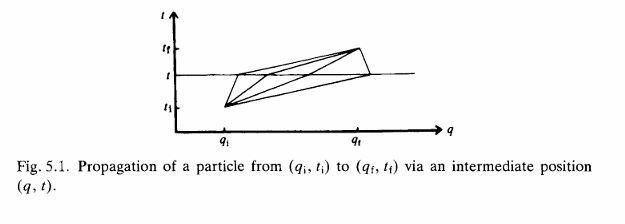
\includegraphics[width=15cm]{figure/fig5-1.png}
\end{figure}

(5.1) を繰り返し適応すると,
\begin{equation*}
    \psi(q_f, t_f) = \int\int K(q_{f}t_{f}; qt)K(qt; q_{i}t_{i})\psi(q_i, t_i)dq_{i}dq,
\end{equation*}
が得られ, そこから
\begin{equation*}
    K(q_{f}t_{f}; q_{i}t_{i}) = \int K(q_{f}t_{f}; qt)K(qt; q_{i}t_{i}) dq \tag{5.2}
\end{equation*}
が導かれるので, $(q_i, t_i)$ から $(q_f, t_f)$ への遷移は, $(q_i, t_i)$ から利用可能なすべての中間点 $q$ への遷移に続いて, $(q, t)$ から $(q_f, t_f)$ への遷移が行われた結果とみなすことができる.\par
図5.2に示す2重スリット実験を考えてみる. 

\begin{figure}[H]
    \centering
    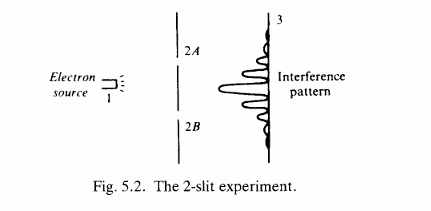
\includegraphics[width=13cm]{figure/fig5-2.png}
\end{figure}

$K(2A; 1)$ は電子が光源 1 からホール 2A を通過する確率振幅であり, $K(3; 2A)$ は電子がホール 2A から検出器 3 へ通過する確率振幅である. 式(5.2)から
\begin{equation*}
    K(3; 1) = K(3; 2A)K(2A; 1) + K(3; 2B)K(2B; 1)
\end{equation*}
であり, スクリーン3の強度パターンは確率 $P(3; 1) = |K(3; 1)|^2$ で与えられるので, 量子論に特徴的な干渉項を含むことは明白. つまり電子はA, Bのホールどちらかを通過したとは言えないことに注意.\\
この全ての可能な経路という概念は, 経路積分の定式化において重要となる.\par
プロパゲータ $K$ が $\braket{q_{f}t_{f}}{q_{i}t_{i}}$ であることを示す. 波動関数 $\psi(q, t)$ は\\
\begin{equation*}
    \psi(q, t) = \braket{q}{\psi t}_{S}
\end{equation*}
であり, Schr\"{o}dinger描像の状態ベクトル $\ket{\psi t}_{S}$ は Hesenberg 描像の状態ベクトル $\ket{\psi}_{H}$ と以下で関係する.
\begin{equation*}
    \ket{\psi t}_{S} = e^{-iHt/\hbar}\ket{\psi}_{H}
\end{equation*}
明らかに「移動方向」と呼べるベクトルを定義する. \textcolor{blue}{$q$ に時間依存性を移す操作なので 'moving flame'}
\begin{equation*}
    \ket{qt} = e^{iHt/\hbar}\ket{q} \tag{5.3}
\end{equation*}
これにより
\begin{equation*}
    \psi(q, t) = \braket{qt}{\psi}_{H} \tag{5.4}
\end{equation*}
となる. 状態ベクトルの完全性 $\displaystyle \left( \int \ket{q_i t_i}\bra{q_i t_i}dq_i = I \right) $ より
\begin{equation*}
    \braket{q_{f}t_{f}}{\psi} = \int \braket{q_{f}t_{f}}{q_{i}t_{i}}\braket{q_{i}t_{i}}{\psi}dq_{i}
\end{equation*}
と書くことができて, 式(5.4)を用いて次のように書くことができる.
\begin{equation*}
    \psi(q_{f}, t_{f}) = \int \braket{q_{f}t_{f}}{q_{i}t_{i}}\psi(q_{i}, t_{i})dq_{i}.
\end{equation*}
式(5.1)と比較すると主張通り次の関係が得られる.
\begin{equation*}
    \braket{q_{f}t_{f}}{q_{i}t_{i}} = K(q_{f}t_{f}; q_{i}t_{i}) \tag{5.5}
\end{equation*}
プロパゲータ $K$ は系の量子力学を要約する. 量子力学の通常の定式化では, 初期の波動関数が与えられれば時間依存のSchr\"{o}dinger方程式を解くことによって最終的な波動関数を求めることができる. しかし, この定式化ではプロパゲータが直接解を与える. ここで考えるのは, $\braket{q_{f}t_{f}}{q_{i}t_{i}}$ を経路積分として表現することである.\par
図5.3のように $t_{i}$ と $t_{f}$ の間との時間間隔を (n + 1) 等分したものを $\tau$ とする.

\begin{figure}[H]
    \centering
    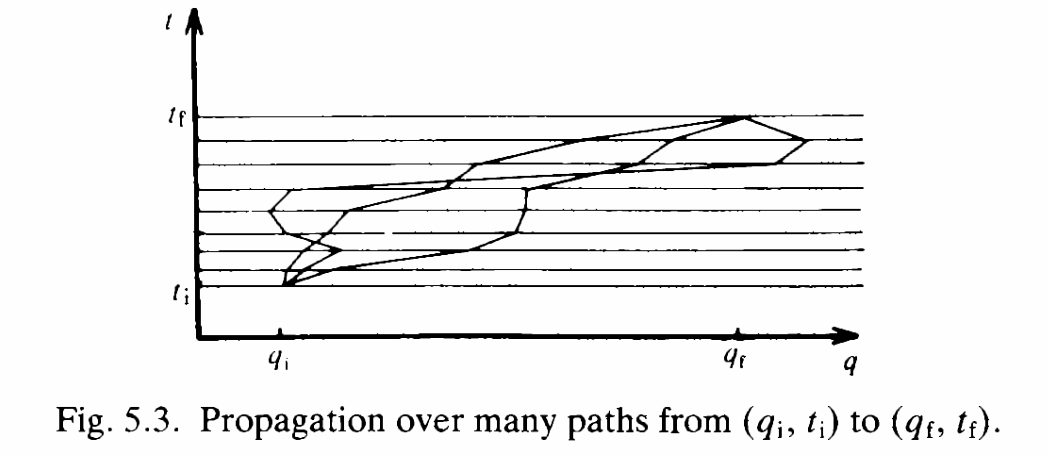
\includegraphics[width=\textwidth]{figure/fig5-3.png}
\end{figure}

式(5.2)は

\begin{equation*}
    \braket{q_{f}t_{f}}{q_{i}t_{i}} = \int \cdots \int dq_{1}dq_{2} \cdots dq_{n} \braket{q_{f}t_{f}}{q_{n}t_{n}}\braket{q_{n}t_{n}}{q_{n-1}t_{n-1}} \cdots \braket{q_{1}t_{1}}{q_{i}t_{i}} \tag{5.6}
\end{equation*}

となり, 積分は全ての可能な「軌跡」に対して行われる. 各区分 $(q_{j}t_{j}; q_{j-1}t_{j-1})$ はより小さな区分に分割される可能性があるため, 通常の意味での軌跡ではなく, 導関数は存在しない. 経路とはマルコフ連鎖である.\\
\textcolor{blue}{マルコフ連鎖は未来の振舞いが現在の値だけで決定され, 過去の振舞いと無関係である(マルコフ性).}\par
ここで経路積分の小さな区間についてプロパゲータを計算してみる. 式(5.3)から
\begin{align*}
    \braket{q_{j+1}t_{j+1}}{q_{j}t_{j}} &= \brakets{q_{j+1}}{e^{-iH\tau}}{q_{j}}\\
    &= \brakets{q_{j+1}}{1 - \frac{i}{\hbar}H\tau + \mathcal{O}(\tau)^{2}}{q_{j}}\\
    &= \delta(q_{j+1} - q_{j}) - \frac{i\tau}{\hbar}\brakets{q_{j+1}}{H}{q_{j}}\\
    &= \frac{1}{2\pi\hbar}\int dp \exp\left[ \frac{i}{\hbar}p(q_{j+1} - q_{j}) \right] - \frac{i\tau}{\hbar}\brakets{q_{j+1}}{H}{q_{j}} \tag{5.7}\\
    &= \frac{1}{h}\int dp \exp\left[ \frac{i}{\hbar}p(q_{j+1} - q_{j}) \right] - \frac{i\tau}{\hbar}\brakets{q_{j+1}}{H}{q_{j}}
\end{align*}
\color{blue}
一般的なデルタ関数の積分表現は $\displaystyle \delta(x) = \frac{1}{2\pi}\int_{-\infty}^{\infty}dp e^{ipx}$. この式は古典的な物理系において単位系に特別な注意を払わずに使うことができるが, 量子系では位置 $q$ と運動量 $p$ が正準共役変数であり, これらはプランク定数 $\hbar$ でスケールされる. 交換関係 $[\hat{q}, \hat{p}] = i\hbar$ は特に運動量が $\hbar$ に依存してスケールされていることを示唆している. このスケールの違いから運動量と位置のフーリエ変換を扱うとき $\hbar$ が重要な役割を果たす.\\
また,運動量空間の状態 $\ket{p}$ と位置空間の状態 $\ket{q}$ のフーリエ変換は $\displaystyle \braket{q}{p} = \frac{1}{2\pi\hbar}e^{\frac{i}{\hbar}pq}$. 運動量の次元は $[p] = [\textrm{位置}]^{-1} \times [\hbar]$ なので, 指数関数の引数を無次元にするために $\hbar$ を導入する必要がある.\\
デルタ関数の積分表現では
\begin{equation*}
    \delta(q_{j+1} - q_{j}) = \frac{1}{2\pi\hbar}\int dp \exp\left[ \frac{i}{\hbar}p(q_{j+1} - q_{j}) \right]
\end{equation*}
となり, $\dfrac{1}{2\pi\hbar}$ はフーリエ変換において位置と運動量の次元を一致させるための正規化係数である. \\
\color{black}
ハミルトニアン $H$ は演算子 $p$ と $q$ の関数である. $H$ が
\begin{equation*}
    H = \frac{p^2}{2m} + V(q) \tag{5.8}
\end{equation*}
の形である特別な場合(実際には $H$ は $p$ の任意の関数と $q$ の任意の関数の組み合わせである)では, (5.7) の行列要素は簡単に計算できる. これより
\begin{equation*}
    \brakets{q_{j+1}}{\frac{p^2}{2m}}{q_{j}} = \int dp' dp \braket{q_{j+1}}{p'}\brakets{p'}{\frac{p^2}{2m}}{p}\braket{p}{q_j}
\end{equation*}
が得られる.\\
\color{blue}
ここで完全性 $\displaystyle \int dp' \ket{p'}\bra{p'}$ を入れたのは $\hat{p}$ が $p$ の固有値として c-number pを出せるため.\\
\color{black}
 $\braket{q_{j+1}}{p'} = (2\pi\hbar)^{-1/2}\exp\left[ \dfrac{i}{\hbar}p'q_{j+1} \right]$ を代入すると式(5.9)が得られる.
\begin{align*}
    \brakets{q_{j+1}}{\frac{p^2}{2m}}{q_j} &= \int \frac{dp' dp}{2\pi\hbar}\exp\left[ \frac{i}{\hbar}(p' q_{j+1} - pq_{j}) \right]\frac{p^2}{2m}\delta(p - p')\\
    &= \int \frac{dp}{h}\exp\left[ \frac{i}{\hbar}p(q_{j+1} - q_{j}) \right]\frac{p^2}{2m}. \tag{5.9}
\end{align*}
ここで注目すべきは式(5.9)の左辺の $p$ は演算子であるのに対し, 右辺の $p$ は数であること. \\
演算子を示すために $\hat{p}$ という表記を使った方が良かっただろう. いずれにせよ, 式(5.9)の右辺が演算子を含まないことは重要な結果である. 同様に,
\begin{align*}
    \brakets{q_{j+1}}{V(q)}{q_j} &= V\left( \frac{q_{j+1} + q_{j}}{2} \right)\braket{q_{j+1}}{q_{j}}\\
    &= V\left( \frac{q_{j+1} + q_{j}}{2} \right)\delta(q_{j+1} - q_{j})\\
    &= \int \frac{dp}{h}\exp\left[ \frac{i}{\hbar}p(q_{j+1} - q_{j}) \right]V(\bar{q}_{j}) \tag{5.10}
\end{align*}
\color{blue}
$\displaystyle V\left( \frac{q_{j+1} + q_j}{2} \right)$としているのは $\braket{q_{j+1}}{q_j}$どちらの固有値でもどうせ後で極限を取って変わらないので中間にしている. また, この表記は後でQFTで扱うときに便利であるという伏線もある.\\
\color{black}
ここで $\bar{q}_{j} = \dfrac{1}{2}(q_{j} + q_{j+1})$ であり, $V(q)$ の左辺は演算子で右辺の積分に含まれる項は演算子ではない. 式(5.9)と式(5.10)から,
\begin{equation*}
    \brakets{q_{j+1}}{H}{q_{j}} = \int \frac{dp}{h} \exp\left[ \frac{i}{\hbar}p(q_{j+1} - q_{j}) \right] H(p, \bar{q}_{j})
\end{equation*}
となり, 式(5.7)から
\begin{equation*}
    \braket{q_{j+1}t_{j+1}}{q_{j}t_{i}} = \frac{1}{\hbar}\int dp_{j} \exp\left\{ \frac{i}{\hbar}[p_{j}(q_{j+1} - q_{j}) - \tau H (p_{j}, \bar{q}_{j})] \right\} \tag{5.11}
\end{equation*}
\color{blue}
\begin{align*}
    \braket{q_{j+1}t_{j+1}}{q_{j}t_{j}} &= \frac{1}{h}\int dp_j \exp\left[ \frac{i}{\hbar}p_{j}(q_{j+1} - q_{j}) \right] - \frac{i\tau}{\hbar}\brakets{q_{j+1}}{H}{q_{j}}\\
    &= \frac{1}{h}\int dp_j \exp\left[ \frac{i}{\hbar}p_{j}(q_{j+1} - q_{j}) \right] - \frac{i\tau}{\hbar} \int \frac{dp_j}{h} \exp\left[ \frac{i}{\hbar}p_{j}(q_{j+1} - q_{j}) \right] H(p_{j}, \bar{q}_{j})\\
    &= \frac{1}{h}\int dp_j \exp\left[ \frac{i}{\hbar}p_{j}(q_{j+1} - q_{j}) \right] \left\{ 1 - \frac{i}{\hbar}\tau H(p_{j}, \bar{q}_{j}) \right\}\\
    &= \frac{1}{h}\int dp_{j} \exp\left[ \frac{i}{\hbar}p_{j}(q_{j+1} - q_{j}) \right] \left( \exp\left[ -\frac{i}{\hbar}\tau H(p_{j}, \bar{q}_{j}) \right) - \mathcal{O}(\tau^2) \right]\\
    &= \int \frac{dp_j}{h}\exp\left[ \frac{i}{\hbar}\left\{ p_j (q_{j+1} - q_j) - \tau H(p_j, \bar{q}_{j}) \right\} \right] \tag{5.11}
\end{align*}
\color{black}
ここで $p_j$ は $t_{j}$ と $t_{j+1}$, 等価的には $q_{j}$ と $q_{j+1}$ の間の運動量である(図5.4参照).

\begin{figure}[H]
    \centering
    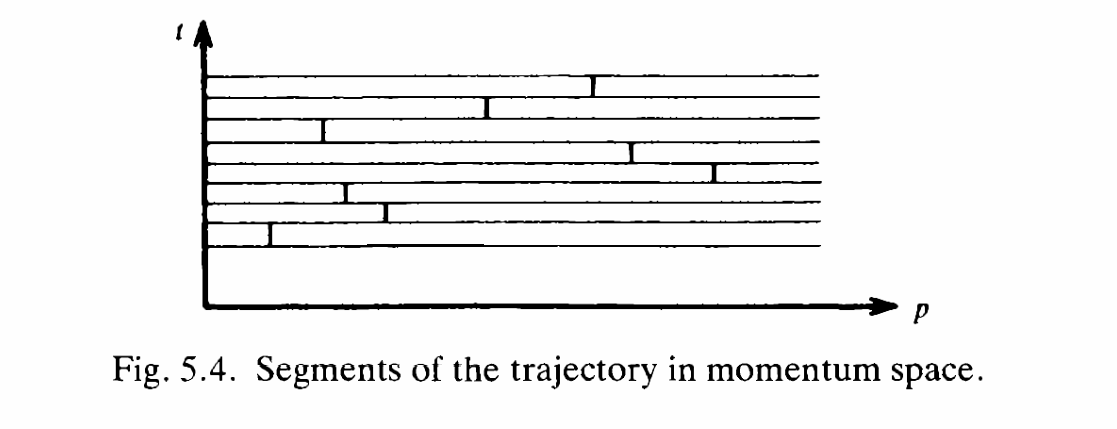
\includegraphics[width=\textwidth]{figure/fig5-4.png}
\end{figure}

これで1つの可能な経路の区間上のプロパゲータが与えられる. これを式(5.6)に代入すると連続体極限($p_{j}$ は $q_{j}$ と $q_{j}$ と $q_{j+1}$ の間の経路に沿った運動量)では $q_{0} = q_{i}, q_{n+1} = q_{f}$ で次のようになる.
\begin{equation*}
    \braket{q_{f}t_{f}}{q_{i}t_{i}} = \lim_{n \rightarrow \infty} \int \prod_{j=1}^{n} dq_{j} \prod_{j=0}^{n}\frac{dp_{j}}{h}\exp\left\{ \frac{i}{\hbar}\sum_{j=0}^{n} [p_{j}(q_{j+1} - q_{j}) - \tau H(p_{j}, \bar{q}_{j})]\right\} \tag{5.12}
\end{equation*}
これは$q(t_i) = q_{i}, q(t_{f}) = q_{f}$ で
\begin{equation*}
    \braket{q_{f}t_{f}}{q_{i}t_{i}} = \int \frac{\mathcal{D}q\mathcal{D}p}{h}\exp\frac{i}{\hbar}\left[ \int_{t_{i}}^{t_{f}} dt [p\dot{q} - H(p, q)] \right] \tag{5.13}
\end{equation*}
という記号で書くことができる. 連続極限では $q$ は $t$ の関数になり\textcolor{blue}{($n \to \infty$ で $\tau \to dt$, 離散状態 $\ket{q}$ が連続 $q(t)$ になる)}, 積分は「汎関数積分」, つまり全ての関数にわたる積分で無次元. 式(5.13)は位相空間における $(q_{i}, t_{i})$ から $(q_{f}, t_{f})$ への遷移振幅に対する経路積分の表現である\color{blue}($\mathcal{D}q\mathcal{D}p$がその積分測度を表している)\color{black}. 各関数 $q(t)$ と $p(t)$ は位相空間の経路を定義する. 前述の通り量子力学に対する一般的なアプローチはSchr\"{o}dinger方程式 $i\hbar\dfrac{d\ket{\psi}}{dt} = \hat{H}\ket{\psi}$ を境界条件に従って解くこと. 経路積分の形式においては遷移振幅の明確な表現を持ち, これは散乱問題に非常に適している. 積分における $p$ と $q$ は古典的な量 (c-number) であり, 演算子 (q-number) ではない. しかし, 無次元積分が数学的定義可能か, つまり収束するかどうか自明でない.\\
言い換えればそれらが存在するかどうかだが, ここでは存在すると仮定する.\\
汎関数積分 $\rightarrow$ Gel'fand $\&$ Yaglom (1960), Kac (1959), Keller $\&$ McLaughlin (1975), Gudder (1979) 参照. \par
遷移振幅には別の形式があり, $H$ が式(5.8)の形を持つ場合に適応される. その場合, $p$-積分を行え,\\
式(5.12)は次のようになる.
\begin{equation*}
    \braket{q_{f}t_{f}}{q_{i}t_{i}} = \lim_{n \rightarrow \infty} \int \prod_{1}^{n}dq_{j}\prod_{0}^{n}\frac{dp_{j}}{h}\exp\left\{ \frac{i}{\hbar}\sum_{0}^{n}\left[ p_{j}(q_{j+1} - q_{j}) - \frac{p^{2}_{j}}{2m}\tau - V(\bar{q}_{j})\tau \right] \right\}
\end{equation*}
$p_{j}$ 積分に
関する限り, これは式(5A.3)と同じ形式であるため(Appendix参照),
\begin{equation*}
    \braket{q_{f}t_{f}}{q_{i}t_{i}} = \lim_{n \rightarrow \infty} \left( \frac{m}{iht} \right)^{(n+1)/2} \int \prod_{1}^{n}dq_{j}\exp\left\{ \frac{i\tau}{\hbar}\sum_{0}^{n}\left[ \frac{m}{2} \left(\frac{q_{j+1} - q_{j}}{\tau}\right)^2 -V \right] \right\}\tag{5.14}
\end{equation*}
となるので, 連続体極限では
\begin{equation*}
    \braket{q_{f}t_{f}}{q_{i}t_{i}} = N\int \mathcal{D}q \exp\left[ \frac{i}{\hbar}\int_{t_i}^{t_f} L(q, \dot{q})dt \right] \tag{5.15}
\end{equation*}
となり, $L = T - V$ は古典的なラグランジアンとなる. $n \rightarrow \infty$ では $N$ は無限になるが, これは問題ではない.\\
\color{blue}
$N$ が無限大でも後で規格化して消すことができるという意味で問題でない.
\color{black}\par
式(5.15)の被積分関数は古典的な作用 $\displaystyle S = \int L dt$ である. 量子力学の公理からこの方程式を導き, ハミルトニアンが 式(5.8)の形をしていると仮定することでこれを証明した. ファインマンの元々のアプローチは式(5.15)を仮定として採用し, そこからSchr\"{o}dinger方程式を証明するものだった. このアプローチの欠点は常に式(5.8)でハミルトニアンが書けるとは限らないので, 式(5.15)が一般的には成り立たないことである.\\
 Lee \& Yang による反例がその例. もし
\begin{equation*}
    L = \frac{\dot{q}^2}{2}f(q)
\end{equation*} 
ならば, これは速度依存のポテンシャルを持つ系を表している. このとき運動量は,
\begin{equation*}
    p = \frac{\partial L}{\partial \dot{q}} = \dot{q}f(q)
\end{equation*}
となり,ハミルトニアンは
\begin{equation*}
    H = p\dot{q} - L = \frac{1}{2}\dot{q}^2 f(q) = \frac{1}{2}\frac{p^2}{f(q)}
\end{equation*}
となる. しかし, これは式(5.8)の形ではない. 式(5.13)式にこの式を代入し, $p$ の積分を実行すると次の式が得られる.
\begin{equation*}
    \braket{q_{f}t_{f}}{q_{i}t_{i}} = N\int \mathcal{D}q \exp\left( \frac{i}{\hbar}S_{\textrm{eff}} \right)
\end{equation*}
ここで $S_{\textrm{eff}}$ は
\begin{equation*}
    S_{\textrm{eff}} = \int dt \left[ L(q, \dot{q}) - \frac{i}{2}\delta(0)\ln f(q) \right].
\end{equation*}
式(5.14)の代わりに有効作用を得る. これは $\displaystyle S = \int L dt$ とは異なる.\par
場の理論におうても同様に, 式(5.13)のような方程式から式(5.15)のような方程式に移行することは一般的にはできないかもしれない. 特に非可換ゲージ理論にはこれが当てはまる. これらの理論については7章で考察する際, 簡単にするために発見的手法なアプローチを採用し, ファインマン則の導出にあたって式(5.15)に類似した方程式を基に議論する.

\subsection*{\textrm{5.2 摂動論と$S$行列}}
本節では経路積分法が散乱過程の計算にどのように使われるのかを示す. 5.3節でラザフォード散乱を考察するが,本ゼミでは5.3節の議論は省略する. 散乱はポテンシャル $V(x)$を介して相互作用する一つの粒子の散乱で, 非相対論的に説明される (この節では座標 $q$ から $x$ への表記変換を行う). 遷移振幅の式は正確に計算できないので, 摂動論を用いる. これはポテンシャル $V(x, t)$ が小さい場合, 厳密に言えば $V(x, t)$ の時間積分が $\hbar$ に比べて小さい場合に有効で次のように書ける.
\begin{equation*}
    \exp\left[ \frac{-i}{\hbar} \int_{t_i}^{t_f} V(x, t)dt \right] = 1 - \frac{i}{\hbar} \int_{t_i}^{t_f} V(x, t)dt - \frac{1}{2!\hbar^2}\left[ \int_{t_i}^{t_f} V(x, t)dt \right]^2 + \cdots \tag{5.16}
\end{equation*} 
これは摂動展開である. プロパゲータ $K(x_{f}t_{f}; x_{i}t_{i})$ の式(5.15)に代入すると (式(5.5)参照), 級数展開
\begin{equation*}
    K = K_0 + K_1 + K_2 + \cdots \tag{5.17}
\end{equation*}
が得られ, その第1項は自由プロパゲータ $K_0$ で以下である.
\begin{align*}
    K_0 &= N \int \left[ \exp \left( \frac{i}{\hbar}S \right) \right]\mathcal{D}x\\
    &= N \int \left[ \exp \left( \frac{i}{\hbar}\int \frac{1}{2}m\dot{x}^2 dt \right) \right]\mathcal{D}x
\end{align*}
これを評価するために,離散形式で書く (式(5.14)参照).\textcolor{blue}{この式(理論)が解けるものなのか知りたい!}
\begin{align*}
    K_0 &= \lim_{n \rightarrow \infty} \left( \frac{m}{ih\tau} \right)^{(n+1)/2} \int_{-\infty}^{\infty} \prod_{j=1}^{n}dx_{j} \exp\left[ \frac{im}{2\hbar\tau}\sum_{j=0}^{n} (x_{j+1} - x_{j})^2 \right]
\end{align*}
この積分の値は, Appendix (5A.4) から
\begin{equation*}
    \textrm{integral} = \frac{1}{(n+1)^{1/2}}\left( \frac{ih\tau}{m} \right)^{n/2} \exp\left[ \frac{im}{2\hbar (n+1)\tau} (x_{f} - x_{i})^2 \right]
\end{equation*}
と知られている. したがって, $(n + 1)\tau = t_{f} - t_{i}$ とおくと自由粒子のプロパゲータは次のようになる.
\begin{equation*}
    K_{0}(x_{f}t_{f}; x_{i}t_{i}) = \left( \frac{m}{ih(t_{f} - t_{i})} \right)^{1/2}\exp\left[ \frac{im(x_{f} - x_{i})^2 }{2\hbar(t_{f} - t_{i})} \right]\hspace{0.5cm} (t_{f} > t_i) \tag{5.18}
\end{equation*}
$t_{f} > t_i$ という条件はプロパゲータにとって非常に重要で, もし $t_{f} < t_i$ の場合, 因果関係によりこの条件は消滅するため次のように書ける. \textcolor{blue}{解けた!!!}
\begin{equation*}
    K_{0}(x_{f}t_{f}; x_{i}t_{i}) = \Theta(t_{f} - t_{i})\left( \frac{m}{ih(t_{f} - t_{i})} \right)^{1/2} \exp\left[ \frac{im(x_{f} - x_{i})^2}{2\hbar(t_{f} - t_{i})} \right] \tag{5.19}
\end{equation*}
$K_{1}$ を計算してみよう. 式(5.14)と式(5.16)から
\begin{equation*}
    K_{1} = \frac{-i}{\hbar}\lim_{n \rightarrow \infty} N^{(n+1)/2}\sum_{i=\textcolor{red}{0}}^{n}\tau\int\exp\left[ \frac{im}{2\hbar\tau}\sum_{j=0}^{n}(x_{j+1} - x_{j})^2 \right] V(x_{i}, t_{i}) dx_1 \cdots dx_{n}
\end{equation*}
であり, ここで $N = \dfrac{m}{ih\tau}$ で $t$ 上の積分を $t_{i}$ 上の総和に置き換えた. $V$ が $x_{i}$ に依存することに注意して, 指数の合計を2つに分割する. 1つは $j=0$ から $j=i-1$ まで, もう1つは $j=i$ から $j=n$ まで. また, $x_{i}$ 上の積分を分離して次を得る.
\begin{align*}
    K_1 = &\lim_{n\rightarrow\infty}\frac{-i}{\hbar}\sum_{i=\textcolor{red}{0}}^{n}\tau\int dx_{i} \left\{ N^{(n-i+1)/2}\int\exp\left[ \frac{im}{2\hbar\tau}\sum_{j=i}^{n}(x_{j+1} - x_{j})^2 \right]dx_{j+1}\cdots dx_{n} \right\}\\
    &\times V(x_{i}, t_{i})\left\{ N^{i/2}\int\exp \left[ \frac{im}{2\hbar\tau}\sum_{j=o}^{i-1}(x_{j+1} - x_{j})^2 \right] dx_1 \cdots dx_{i-1} \right\} 
\end{align*}
中括弧の2つの項は $K_{0}(x_{f}t_{f}; xt)$ と $K_{0}(xt; x_{i}t_{i})$ より, $\displaystyle \lim_{n \to \infty} \sum_{i}^{n}\tau\int dx_{i} \to \int dx dt$ に置き換えると,
\begin{equation*}
    K_{1}(x_{f}t_{f}; x_{i}t_{i}) = -\frac{i}{\hbar}\int_{t_i}^{t_f}dt\int_{-\infty}^{\infty} K_{0}(x_{f}t_{f}; xt)V(x, t)K_{0}(xt; x_{i}t_{i})dx. \tag{5.20}
\end{equation*}
ここで, $t > t_f$ であれば $K_{0}(x_{f}t_{f}; xt)$ がゼロ, $t < t_i$ であれば $K_{0}(xt; x_{i}t_{i})$ はゼロなので, 式(5.20)の積分を $t$ がゼロになるまで実行すると式(5.21)が得られる.
\begin{equation*}
    K_{1}(x_{f}t_{f}; x_{i}t_{i}) = -\frac{i}{\hbar}\int_{-\infty}^{\infty}dt\int K_{0}(x_{f}t_{f}; xt)V(x, t)K_{0}(xt; x_{i}t_{i})dx. \tag{5.21}
\end{equation*}
これが自由プロパゲータに対する1次補正である. 同様の方法で2次補正(式(5.22))を証明できる.
\begin{align*}
    K_{2}(x_{f}t_{f}; x_{i}t_{i}) = &\left( \frac{-i}{\hbar} \right)^2 \int_{-\infty}^{\infty} dt_1 \int_{-\infty}^{\infty} dt_2 \int_{-\infty}^{\infty} dx_1 \int_{-\infty}^{\infty}dx_2 K_{0}(x_{f}t_{f}; x_{2}t_{2})V(x_{2}, t_{2}) \\
    & \times K_{0}(x_{2}t_{2}; x_{1}t_{1})V(x_{1}, t_{1})K_{0}(x_{1}t_{1}; x_{i}t_{i}) \tag{5.22}
\end{align*}
\textcolor{red}{証明の計算をやっておく}\\
同様の表現が展開式(5.17)における全ての $K_n$ に対して成り立つので, 次のように書ける.
\begin{align*}
    K(x_f t_f; x_i t_i) = &K_0(x_f t_f; x_i t_i) - \frac{i}{\hbar} \int K_0(x_f t_f; x_1 t_1)V(x_1, t_1)K_0(x_1 t_1; x_i t_i)dx_1 dt_1\\
    & - \frac{1}{\hbar^2}\int K_0(x_f t_f; x_1 t_1)V(x_1, t_1)K_0(x_1 t_1; x_2 t_2)V(x_2, t_2)\\
    & \times K_0(x_2 t_2; x_i t_i)dx_1 dx_2 dt_1 dt_2 + \cdots. \tag{5.23}
\end{align*}
これは $K$ における摂動級数に対する解であり, ボルン展開と呼ばれ図5.5のように視覚化できる.
\begin{figure}[H]
    \centering
    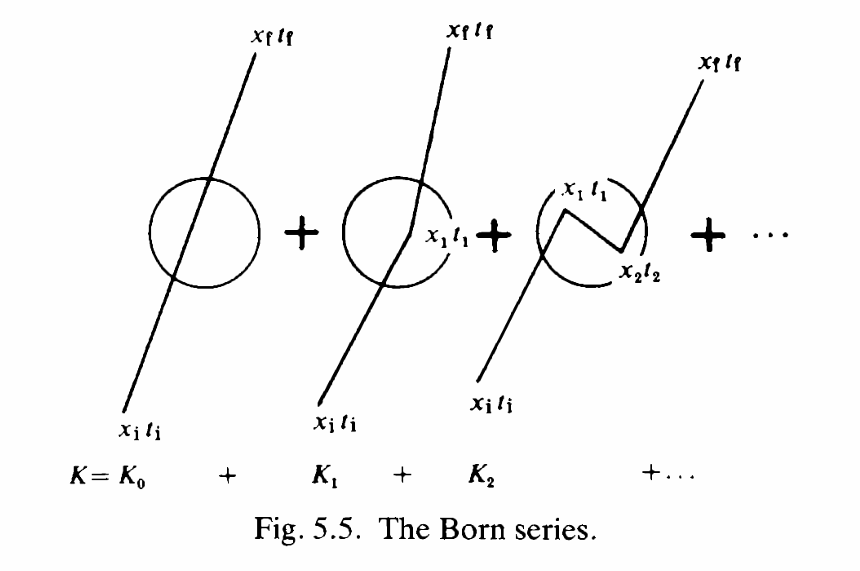
\includegraphics[width=\textwidth]{figure/fig5-5.png}    
\end{figure}
$K_0$ は波動関数が $x_{i}t_{i}$ から $x_{f}t_{f}$ まで自由に伝播することを, $K_1$ はポテンシャル $V$ との1回の相互作用を含む伝播を表し, 以下同様に進む.\par
式(5.22)の注目すべき特徴は, 式(5.16)に存在する $\dfrac{1}{2!}$ の因子を含まないことで, その理由を以下で示す.\\
ポテンシャル $V$ との2回の相互作用は異なる時点で発生するが, 識別ができないため次のように書く.
\begin{align*}
    \frac{1}{2!}\int V(t')V(t'') dt' dt'' &= \frac{1}{2!} \int \left[\theta(t' - t'')V(t')V(t'') + \theta(t'' - t')V(t')V(t'')\right]dt'dt''\\
    &= \theta(t_1 - t_2)V(t_1)V(t_2) dt_1 dt_2. \tag{5.24}
\end{align*}
同様に $K_n$ の式には $\dfrac{1}{n!}$ の因子は存在しない. 次にプロパゲータ $K_0$ がSchr\"{o}dinger方程式のグリーン関数でしかないことを示す. そのためにボルン展開(式(5.23))を式(5.1), $\displaystyle \psi(q_f, t_f) = \int K(q_{f}t_{f}; q_{i}t_{i})\psi(q_i, t_i)dq_i$ に代入する. これにより,
\begin{align*}
    \psi(\mathbf{x}_f t_f) &= \int K(\mathbf{x}_f t_f; \mathbf{x}_i t_i)\psi(\mathbf{x}_i t_i)d\mathbf{x}_i\\
    &= \int K_0(\mathbf{x}_f t_f; \mathbf{x}_i t_i)\psi(\mathbf{x}_i t_i)d\mathbf{x}_i\\
    &\quad - \frac{i}{\hbar}\int K_0(\mathbf{x}_f t_f; \mathbf{x}_1 t_1)V(\mathbf{x}_1 t_1)K_0(\mathbf{x}_1 t_1; \mathbf{x}_i t_i)\psi(\mathbf{x}_i t_i)d\mathbf{x}_i d\mathbf{x}_1 dt_1 + \cdots. \tag{5.25}
\end{align*}
\textcolor{blue}{これまで簡単に1次元で考えてきたが, 3次元空間に戻す. そのためベクトル表記 $\mathbf{x}$ となっていることに注意.}\\
式(5.25)の級数が収束すると仮定すると, 省略された項の影響は $K_0$ を完全なプロパゲータ $K$ に修正するだけなので次のようになる.
\begin{equation*}
    \psi(\mathbf{x}_f t_f) = \int K_0(\mathbf{x}_f t_f; \mathbf{x}_i t_i)\psi(\mathbf{x}_i t_i)d\mathbf{x}_i - \frac{i}{\hbar}\int K_0(\mathbf{x}_f t_f; \mathbf{x} t)V(\mathbf{x}, t)\psi(\mathbf{x}t)d\mathbf{x} dt. \tag{5.26}
\end{equation*}
\color{blue}
$\psi(x_1, t_1)$でポテンシャルの添字が2になる理由を聞いておく
\color{black}
この式は厳密であり, $\psi$ に対する積分方程式である. いま, 遠方の過去 $t_i \rightarrow -\infty$ では $\psi$ は平面波 $\phi$ となり, 式(5.26)の右辺初項も平面波になる. これは $\psi(\mathbf{x}_f t_f)$ の自由な伝播に由来するためである. したがって,
\begin{equation*}
    \psi(\mathbf{x}_f t_f) = \phi(\mathbf{x}_f t_f) - \frac{i}{\hbar}\int K_0(\mathbf{x}_f t_f; \mathbf{x} t)V(\mathbf{x}, t) \phi(\mathbf{x} t)d\mathbf{x} dt. \tag{5.27}
\end{equation*}
と書くことができる. ここで$\psi(\mathbf{x}_f t_f)$ は Schr\"{o}dinger方程式を満たす.
\begin{equation*}
    \frac{\hbar^2}{2m}\nabla_{\mathbf{x}}^2 \psi(\mathbf{x}_f t_f) + i\hbar \frac{\partial}{\partial t_f} \psi(\mathbf{x}_f t_f) = V(\mathbf{x}_f t_f)\psi(\mathbf{x}_f t_f). \tag{5.28}
\end{equation*}
次に $\phi(\mathbf{x}_f t_f)$ が自由粒子 $V = 0$ であるとすると $K_0$ は次を満たす.
\begin{equation*}
    \frac{\hbar^2}{2m}\nabla_{\mathbf{x}}^2 K_0(\mathbf{x}_f t_f; \mathbf{x} t) + i\hbar \frac{\partial}{\partial t_f} K_0(\mathbf{x}_f t_f; \mathbf{x} t) = i\hbar \delta(\mathbf{x}_f - \mathbf{x})\delta(t_f - t) \tag{5.29}
\end{equation*}
これは式(5.28)のグリーン関数の方程式である. $\delta(t_f - t)$ の存在は式(5.19)の定義から期待されるものであり, $K_0$ は主張通りSchr\"{o}dinger方程式のグリーン関数でしかないことが分かる.
\color{blue}

\color{black}
散乱振幅の計算に進む. 散乱過程の測定では, 実験条件として粒子は$t = -\infty$のとき自由であり, 散乱して $t = +\infty$ で再び自由になると仮定する. ただこの仮定には困難がある. なぜなら自由粒子 (すなわち, 確定したエネルギーと運動量を持つ粒子) は平面波として記述され, 全ての空間と時間に広がるため. したがって, 相互作用ポテンシャル $V(\mathbf{x})$ が含まれる領域でも粒子は常に自由である必要がある. この問題を解決するために Adiabatic 仮説(断熱的仮説)が導入される. (ポテンシャル $V$ は徐々にオンおよびオフにされ, $t = -\infty$ で $V = 0$ となり, $t = +\infty$ でも粒子は自由である. オンおよびオフを急速に切り替えてはいけない.) これはフーリエ変換を通じて, 散乱中心での $V$ の時間依存性がエネルギーの放出または吸収を伴わないことを意味する.\par
散乱問題に戻ると, 初期条件は $\psi$ が平面波であると仮定する:
\begin{equation*}
    \psi_{\textrm{in}}(\mathbf{x}_i,t_i) = \textrm{plane wave}.
\end{equation*}
$V \to 0$ を $t \to -\infty$ の時とし, また $t_i$ がさらに過去であると仮定する.\\
最初のボルン近似を(5.25)式に適用すると次のようになる.
\begin{align*}
    \psi^{(+)}(\mathbf{x}_{f} t_{f}) = \int &K_0(\mathbf{x}_f t_f; \mathbf{x}_i t_i) \psi_{\textrm{in}}(\mathbf{x}_i t_i) d\mathbf{x}_i\\
    &- \frac{i}{\hbar} \int K_0(\mathbf{x}_f t_f; \mathbf{x}t)V(\mathbf{x},t)K_0(\mathbf{x}t;\mathbf{x}_i t_i)\psi_{\textrm{in}}(\mathbf{x}_i t_i)d\mathbf{x} d\mathbf{x}_i dt. \tag{5.30}
\end{align*}
$\psi^{(+)}(\mathbf{x}_f,t_f)$ の上付きプラス記号は, これが $t = -\infty$ で自由な波に対応することを示し「遅延」プロパゲータ $K_0(\mathbf{x}_f t_f; \mathbf{x}'t')$ を含む. この $K_0$ は $t' > t$ の場合に消える. また, $\psi^{(-)}(\mathbf{x}_1 t_1)$ は $t = +\infty (\psi_{\textrm{out}})$ で自由になる波として書くことも同様に可能で, 「進行」プロパゲータ $K_0(\mathbf{x} t; \mathbf{x}'t')$ を含み, これは $t' < t$ の場合に消える.\par
我々は明確な運動量を持つ最終状態の粒子を検出する振幅に興味がある. これは散乱振幅 $S$ と呼ばれ, 波動関数の重なりとして表される.
\begin{align*}
    S &= \int \psi_{\textrm{out}}^{*}(\mathbf{x}_f t_f)\psi^{(+)}(\mathbf{x}_f t_f)d\mathbf{x}_f\\
    &= \int \psi_{\textrm{out}}^{*}(\mathbf{x}_f t_f)K_0(\mathbf{x}_f t_f; \mathbf{x}_i t_i)\psi_{\textrm{in}}(\mathbf{x}_i t_i)d\mathbf{x}_i d\mathbf{x}_f\\
    &\quad -\frac{i}{\hbar} \int \psi_{\textrm{out}}^{*}(\mathbf{x}_f t_f)K_0(\mathbf{x}_f t_f; \mathbf{x}t)V(\mathbf{x},t)K_0(\mathbf{x}t; \mathbf{x}_i t_i)\psi_{\textrm{in}}(\mathbf{x}_i t_i)d\mathbf{x}_f d\mathbf{x} d\mathbf{x}_i dt\\
    &= \int \psi_{\textrm{out}}^{*}(\mathbf{x}_f t_f)\phi(\mathbf{x}_f t_f)d\mathbf{x}_f -\frac{i}{\hbar} \int \psi_{\textrm{out}}^{*}(\mathbf{x}_f t_f)K_0 (\mathbf{x}_f t_f; \mathbf{x}t)\\
    &\quad \times V(\mathbf{x}, t)K_0 (\mathbf{x} t; \mathbf{x}_i t_i)\psi_{\textrm{in}}(\mathbf{x}_i t_i)d\mathbf{x}_f d\mathbf{x} d\mathbf{x}_i dt. \tag{5.31}
\end{align*}
ここで $\phi(\mathbf{x}_f t_f)$ は $\psi(\mathbf{x}_i t_i)$ と同じく平面波である.\\
初期運動量と最終運動量を $\mathbf{p}_i = \hbar \mathbf{k}_i$, $\mathbf{p}_f = \hbar \mathbf{k}_f$ とすると, box normalization (箱正規化) により以下となる.
\begin{align*}
    \psi_{\textrm{in}}(\mathbf{x}t) &= \frac{1}{\sqrt{\tau}} \exp{\left[ \frac{i}{\hbar}(\mathbf{p}_i \cdot \mathbf{x} - E_i t)\right]},\\
    \psi_{\textrm{out}}(\mathbf{x}t) &= \frac{1}{\sqrt{\tau}} \exp{\left[ \frac{i}{\hbar}(\mathbf{p}_f \cdot \mathbf{x} - E_f t)\right]} \tag{5.32}
\end{align*}
ここで, $E = \dfrac{p^2}{2m}$ であり, $\tau$ は箱の体積を表します(もちろんこれは任意の値である).\\
\textcolor{blue}{box normalizationは量子力学や場の量子論で使われる手法の一つ. 連続的な運動量や位置空間における波動関数の正規化を扱うための便宜的な方法. 具体的には無限に広がる空間で波動関数を取り扱うのは難しいため, 空間を有限な「箱」に閉じ込め, その中で波動関数を正規化する考え方.\\
計算を有限な体積で行い, その後無限体積の極限を取ることで連続的な波数空間での正規化や積分を扱うことが可能になる. これにより平面波のような波動関数でも適切に扱うことができる.}\\
式(5.32)を式(5.31)の初項に代入し,
\begin{equation*}
    \int e^{i \mathbf{q} \cdot \mathbf{x}} d\mathbf{x} = (2\pi)^3 \delta(\mathbf{q})
\end{equation*}
を用い, 便宜上 $\tau = (2\pi)^3$ とおくと、次のようになる.
\begin{align*}
    S_{fi} = \delta(\mathbf{k}_i - \mathbf{k}_f) - \frac{i}{\hbar} \int \psi_{\textrm{out}}(\mathbf{x}_f t_f)K_0(\mathbf{x}_f t_f; \mathbf{x}t)V(\mathbf{x},t)K_0(\mathbf{x}t; x_i t_i)\psi_{\textrm{in}}(\mathbf{x}_i t_i)d\mathbf{x}_f d\mathbf{x} d\mathbf{x}_i dt. \tag{5.33}
\end{align*}
散乱振幅は行列 $S$ の1つの要素, すなわち $S$ 行列 (または散乱行列) の要素として解釈される. 行列 $S$ の (fi) 要素は式(5.33)で示されている. 初項は運動量保存に対応し, 相互作用がない場合には単位行列 $S$ を与える. 実際の相互作用は式(5.33)の第2項で表される. そして特定の「入射」状態から特定の「出射」状態に対して得られる振幅は次のように与えられる.
\begin{equation*}
    A = -\frac{i}{\hbar} \int \psi_{\textrm{out}}^{*}(\mathbf{x}_f t_f)K_0(\mathbf{x}_f t_f; \mathbf{x}t)V(\mathbf{x},t)K_0(\mathbf{x}t; \mathbf{x}_i t_i)\psi_{\textrm{in}}(\mathbf{x}_i t_i)d\mathbf{x}_f d\mathbf{x} d\mathbf{x}_i dt. \tag{5.34}
\end{equation*}
これで自由プロパゲータ $K_0$ と相互作用ポテンシャル $V$ に関する散乱振幅の表現を得た. 式(5.34)は散乱振幅を計算する簡単な規則に置き換え可能で, この規則はファインマンルールとして知られている.\par
散乱振幅 (5.34)は次の図で表すことができる.
\begin{figure}[H]
    \centering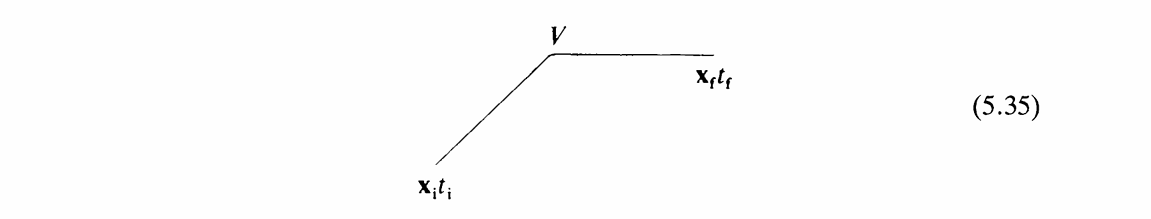
\includegraphics[width=\textwidth]{figure/eq5-35.png}
\end{figure}
この図を散乱振幅の表現に変換するための規則は, 以下と対応させることで要約できることは明らかである.
\begin{figure}[H]
    \centering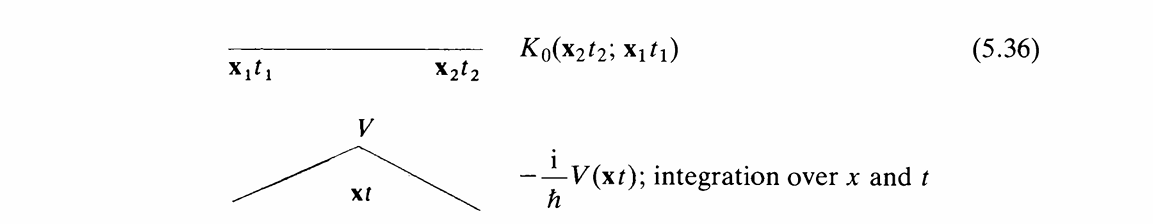
\includegraphics[width=\textwidth]{figure/eq5-36.png}
\end{figure}
さらに図の両端で $\psi_{\textrm{in}}$ と $\psi_{\textrm{out}}^{*}$ を掛け合わせて関連する2つの空間変数で積分する.\\
したがって2次過程に対する振幅
\begin{figure}[H]
    \centering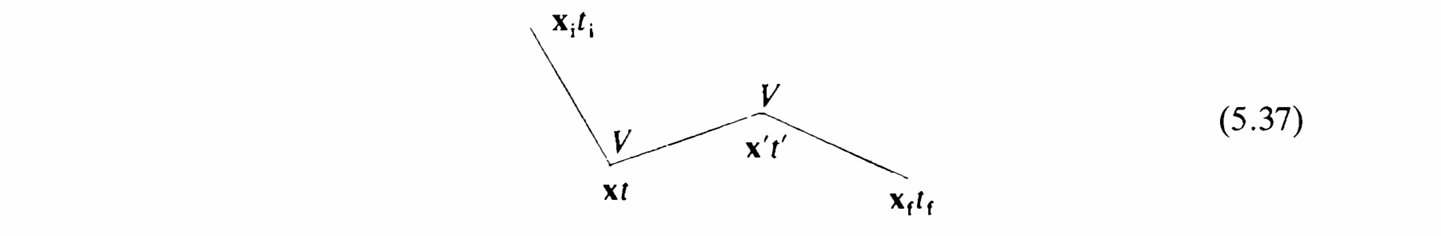
\includegraphics[width=\textwidth]{figure/eq5-37.png}
\end{figure}
は次のようになる.
\begin{align*}
    A^{(2)} &= \left( -\frac{i}{\hbar} \right)^2 \int \psi_{\textrm{out}}^{*}(\mathbf{x}_f t_f) K_0(\mathbf{x}_f t_f; \mathbf{x}'t') V(\mathbf{x}',t')K_0(\mathbf{x}'t'; \mathbf{x}t) V(\mathbf{x},t)\\
    & \quad \times  K_0(\mathbf{x}t; \mathbf{x}_i t_i) \psi_{\textrm{in}}(\mathbf{x}_i t_i) d\mathbf{x}_i d\mathbf{x} dt d\mathbf{x}' dt' d\mathbf{x}_f.
    \end{align*}
    これらの式(5.36)はファインマンルールと呼ばれる. 我々が現在取り扱っている非相対論的な量子力学ではこれらの規則はほとんど必要ないが, 場の理論では計算をする際に非常に便利である. 次の章で考察される非摂動的理論ではこれらは大いに役立つ.\par
    式(5.36)は座標空間で書かれている. しかし, 多くの計算においては運動量空間で作業する方が便利である. この節の残りでは運動量空間における対応するファインマンルールを導出する. 運動量空間において $\mathcal{K}(\mathbf{p}_1 t_1; \mathbf{p}_0 t_0)$ は, 時間 $t_0$ において運動量 $\mathbf{p}_0$ を持つ粒子が時間 $t_1$ で運動量 $\mathbf{p}_1$ を持つように観測される確率振幅であるとする. これは次の式で与えられる.
\begin{equation*}
        \mathcal{K}(\mathbf{p}_1 t_1; \mathbf{p}_0 t_0) = \int \exp \left( -\frac{i}{\hbar} \mathbf{p}_1 \cdot \mathbf{x}_1 \right) K_0(\mathbf{x}_1 t_1; \mathbf{x}_0 t_0) \exp \left( \frac{i}{\hbar} \mathbf{p}_0 \cdot \mathbf{x}_0 \right) d\mathbf{x}_0 d\mathbf{x}_1. \tag{5.38}
\end{equation*}
自由プロパゲータ $K_0(\mathbf{x}_1 t_1; \mathbf{x}_0 t_0)$ は式(5.19)の3次元の一般化によって次のように与えられる.
\begin{equation*}
    K_0(\mathbf{x}_1 t_1; \mathbf{x}_0 t_0) = \theta(t_1 - t_0) \left( \frac{m}{i\hbar(t_1 - t_0)} \right)^{3/2} \exp \left[ \frac{im}{2\hbar} \frac{(\mathbf{x}_0 - \mathbf{x}_1)^2}{(t_1 - t_0)} \right]. \tag{5.39}
\end{equation*}
したがって, $\mathcal{K}(p_1 t_1; p_0 t_0)$ は次のようになる.
\begin{align*}
    \mathcal{K}(p_1 t_1; p_0 t_0) &= \theta(t_1 - t_0) \left( \frac{m}{i\hbar(t_1 - t_0)} \right)^{3/2} \int \exp\left[ \frac{i}{\hbar}(\mathbf{p}_0 \cdot \mathbf{x}_0 - \mathbf{p}_1 \cdot \mathbf{x}_1) \right]\\
    &\quad \times \exp\left[ \frac{im}{2\hbar} \frac{(\mathbf{x}_0 - \mathbf{x}_1)^2}{(t_1 - t_0)} \right]d\mathbf{x}_0 d\mathbf{x}_1.
\end{align*}
この積分を評価するために以下の変数を導入する.
\begin{equation*}
    \mathbf{x} = \mathbf{x}_0 - \mathbf{x}_1, \quad \mathbf{X} = \mathbf{x}_0 + \mathbf{x}_1, \quad \mathbf{p} = \mathbf{p}_0 - \mathbf{p}_1, \quad \mathbf{P} = \mathbf{p}_0 + \mathbf{p}_1
\end{equation*}
すると, 
\begin{equation*}
    2(\mathbf{p}_0 \cdot \mathbf{x}_0 - \mathbf{p}_1 \cdot \mathbf{x}_1) = \mathbf{P} \cdot \mathbf{x} + \mathbf{p} \cdot \mathbf{X}
\end{equation*}
となる. 変数変換のヤコビアンは $\left( \dfrac{1}{2} \right)^3 = \dfrac{1}{8}$ なので, 次の式が得られる.
\begin{equation*}
    \mathcal{K}_0(\mathbf{p}_1 t_1; \mathbf{p}_0 t_0) = \theta(t_1 - t_0) \left( \frac{2\alpha}{i} \right)^{3/2} \frac{1}{8}\int \exp \left( \frac{i}{2\hbar} \mathbf{} \cdot \mathbf{X} \right)d\mathbf{X} \times  \int \exp \left( \frac{i}{2\hbar} \mathbf{P} \cdot \mathbf{x} \right)e^{i\alpha\mathbf{x}^2}  d\mathbf{x}
\end{equation*}
ここで, $\alpha = \dfrac{m}{2\hbar(t_1 - t_0)}$ である. 最初の積分は $(2\pi\hbar)^3 \delta\mathbf{p} = (2\pi\hbar)^3 \delta(\mathbf{p}_0 - \mathbf{p}_1)$ となるので,
\begin{equation*}
    \mathcal{K}_0(\mathbf{p}_1  t_1; \mathbf{p}_0 t_0) = (2\pi \hbar)^3 \theta(t_1 - t_0) \delta(\mathbf{p}_0 - \mathbf{p}_1) \left( \frac{2\alpha}{i} \right)^{3/2} \int \exp \left( \frac{i}{2\hbar} \mathbf{P} \cdot \mathbf{x} + i\alpha\mathbf{x}^2 \right) d\mathbf{x}.
\end{equation*}
この式は式(5A.3)で評価することができ, 次の式を与える.
\begin{equation*}
    \mathcal{K}_0(\mathbf{p}_1  t_1; \mathbf{p}_0 t_0) = (2\pi \hbar)^3 \theta(t_1 - t_0) \delta(\mathbf{p}_0 - \mathbf{p}_1) \exp \left[ -\frac{i\mathbf{P}^2 (t_1 - t_0)}{8m\hbar} \right].
\end{equation*}
デルタ関数は $\mathbf{p}_1 = \mathbf{p}_0$ を示唆し, 運動量が保存されているときのみ伝播が生じることが分かる. さらに $\mathbf{P}^2 = 4\mathbf{p}_{0}^2$ を得るので、最終的に次のようになる.
\begin{equation*}
    \mathcal{K}_0(\mathbf{p}_1  t_1; \mathbf{p}_0 t_0) = (2\pi \hbar)^3 \theta(t_1 - t_0) \delta^3(\mathbf{p}_0 - \mathbf{p}_1) \exp \left( \frac{i\mathbf{p}_{0}^2 (t_1 - t_0)}{2m\hbar} \right) \tag{5.40}
\end{equation*}
このプロパゲータは既に述べたように, 時間 $t_1$ で運動量 $p_1$ を持つ粒子が時間 $t_0$ で運動量 $\mathbf{p}_0$ を持っていたときの振幅を与える. この量のフーリエ変換は当然 $\mathcal{K}_0(\mathbf{x}_1 t_1; \mathbf{x}_0 t_0)$ であり, 式(5.38)の逆数で与えられ, 式(5.40)を代入すると次の式を得る.
\begin{align*}
    K_0(\mathbf{x}_1 t_1; \mathbf{x}_0 t_0) &= \frac{1}{(2\pi \hbar)^6} \int \exp \left( \frac{i}{\hbar} \mathbf{p}_1 \cdot \mathbf{x}_1 \right) \mathcal{K}_0(\mathbf{p}_1  t_1; \mathbf{p}_0 t_0) \exp \left( -\frac{i}{\hbar} \mathbf{p}_0 \cdot \mathbf{x}_0 \right) d\mathbf{p}_1 d\mathbf{p}_0\\
    &= \theta(t_1 -t_0)\frac{1}{(2\pi\hbar)^3}\int\exp\left\{ \frac{i}{\hbar}\left[ \mathbf{q} \cdot (\mathbf{x}_1 - \mathbf{x}_0) - \frac{\mathbf{q}^2}{2m}(t_1 - t_0) \right] \right\}d\mathbf{q} \tag{5.41}
\end{align*}
この式を次の節のクーロン散乱計算に応用するが, 今回はパス.\par
最後に時間依存のフーリエ変換を行い, 時間と空間を対称的に扱うようにする. \\
これは相対論的な例に必要で, プロパゲータは
\begin{align*}
    k_0(\mathbf{p}_1 E_1; \mathbf{p}_0 E_0) &= \int \exp \left( \frac{i}{\hbar} E_1 t_1 \right) \mathcal{K}_0(\mathbf{p}_1 t_1; \mathbf{p}_0 t_0) \exp \left( - \frac{i}{\hbar} E_0 t_0 \right) dt_0 dt_1 \\
    &= (2\pi \hbar)^3 \delta(\mathbf{p}_0 - \mathbf{p}_1) \theta(\tau) \exp \left( - \frac{ip_1^2}{2m\hbar} \tau \right) \\
    &\quad \times \exp \left[ \frac{i}{\hbar} (E_1 t_1 - E_0 t_0) \right] dt_0 dt_1 \tag{5.42}
\end{align*}
ここで $\tau = t_1 - t_0$ である. $\tau$ と $t_0$ を独立変数として扱うと次のようになる.
\begin{align*}
    \mathcal{K}_0(\mathbf{p}_1 E_1; \mathbf{p}_0 E_0) &= (2\pi \hbar)^3 \delta(\mathbf{p}_0 - \mathbf{p}_1) \int_{-\infty}^{\infty} \exp \left[ \frac{i}{\hbar} (E_1 - E_0) t_0 \right] dt_0 \\
    &\quad \times \int_{-\infty}^{\infty} \theta(\tau) \exp \left[ \frac{i}{\hbar} \left( E_1 - \frac{p_1^2}{2m} \right) \tau \right] d\tau.
\end{align*}
最初の積分は $(2\pi \hbar) \delta(E_1 - E_0)$ である. 2つ目の積分に含まれる $\theta(\tau)$ 関数の存在により,
\begin{equation*}
    \int_0^{\infty} e^{i\omega\tau} d\tau
\end{equation*}
という形式になり, $\omega$ が実数である場合, 積分は収束しない. 収束させるためには $\omega$ を $\omega + i\epsilon$ と置き換える. ここで $\epsilon$ は小さく正の値である. この積分の値は $\dfrac{i}{(\omega + i\epsilon)}$ となる. $\omega$ を代入すると次の式が得られる.
\begin{equation*}
    k_0(\mathbf{p}_1 E_1; \mathbf{p}_0 E_0) = (2\pi \hbar)^4 \delta(\mathbf{p}_0 - \mathbf{p}_1) \delta(E_0 - E_1) \frac{i\hbar}{E_1 - \frac{p_1^2}{2m} + i\epsilon}. \tag{5.43}
\end{equation*}
予想された通り, このプロパゲータはエネルギー保存および運動量保存を示す. $\epsilon \to 0$ の極限は式(5.43)において理解されるべきである. ここで重要な点は波動力学で記述される粒子に対して, エネルギー $E$ が必ずしも $\dfrac{p^2}{2m}$ ではないこと. $E$と$p$は独立した変数である ( $t$ および $x$ 空間からフーリエ変換を定義するために使用される). これは量子論で消滅するサイズを持つ波束として記述される古典的な点粒子に対してのみ適用され, $E = \dfrac{p^2}{2m}$となる. この極限では上のプロパゲータは極を持つ. しかし, 一般的には任意の $E$ および $p$ に対して伝播が生じる.\par
次にポテンシャル $V(\mathbf{x}, t)$ のフーリエ変換を導入すると次のように書くことができる.
\begin{equation*}
    V(\mathbf{x}, t) = \int \exp \left( - \frac{i}{\hbar} (\mathbf{q} \cdot \mathbf{x} - Wt) \right) v(\mathbf{q}, W) d\mathbf{q} dW \tag{5.44}
\end{equation*}
すると振幅(5.34)は $k_0$ と $\upsilon$ で表され, 運動量空間
\begin{figure}[H]
    \centering
    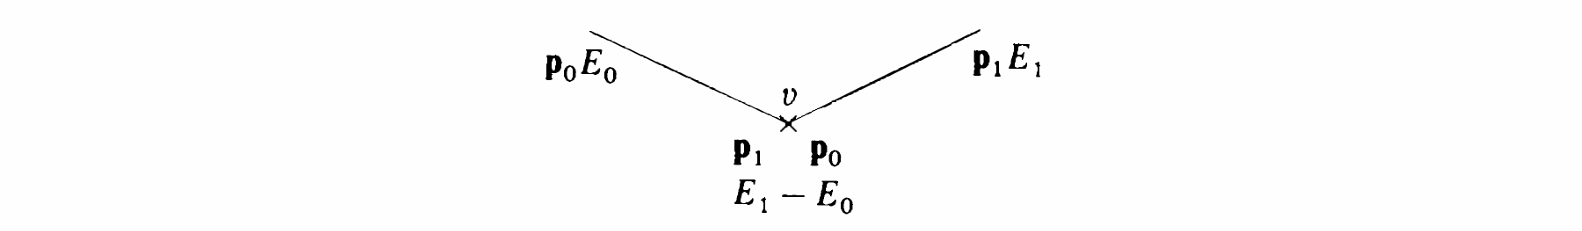
\includegraphics[width=\textwidth]{figure/figB5-45.png}
\end{figure}
で要約され, その意味はファインマンルールで与えられる.
\begin{figure}[H]
    \centering
    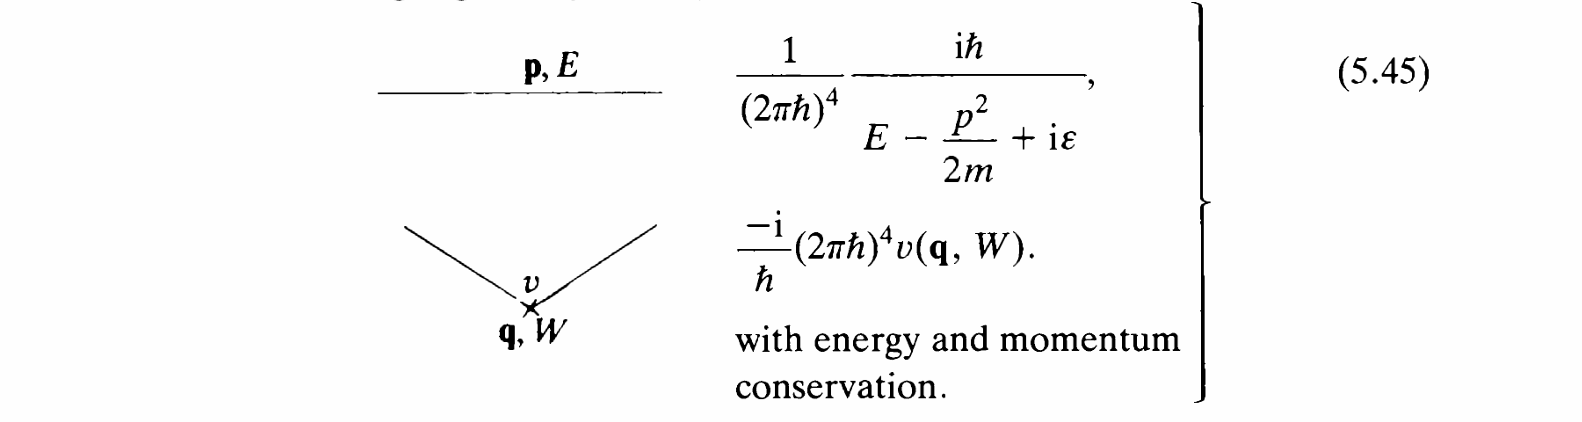
\includegraphics[width=\textwidth]{figure/eq5-45.png}
\end{figure}

\end{document}